\header{
    \headtitle{Le vin gaulois} \label{le-vin-gaulois}
    %
    \insertComment{Appelé le chant du glaive, il s'agit d'un chant celte du VIe siècle.}{En 578 les vénètes conquirent le vannetais aux dépens des francs.}
}

\enluminure{3}{\href{https://www.youtube.com/watch?v=4zKOLGwku8o}{V}}~\\
$\left.\begin{tabular}{l}
\hspace {-0.4cm}
\textsc{ive} le vieux vin de vigne 
\\
\hspace{-0.4cm}
Le vieux vin gaulois
\end{tabular}\right\rbrace$ bis
\\\\\textbf{Refrain :}
\\Tan, tan, terre et ciel
\\Chêne, feu, rouge soleil
\\Tan, tan, glaive clair
\\Flots de sang vermeil
\bisdoublespace{Mieux que bière ou vin de pomme}
{Mieux vaut vin gaulois!}
\bisdoublespace{C'est le sang gaulois qui coule ~~~~}
{C'est le sang gaulois!}
\bisdoublespace{Sang et vin mêlés ruissellent ~~~~~~}
{Sang et vin gaulois!}
\bisdoublespace{Glaive, maître des batailles ~~~~~~~}
{Glaive, honneur à toi!}
\bisdoublespace{C'est le glaive bleu qui frappe ~~~~}
{C'est le glaive roi!}
\bisdoublespace{Qu'au soleil le fer flamboie ~~~~~~~~}
{Comme l'arc en ciel!}

\bigskip
\begin{center}
\centering
    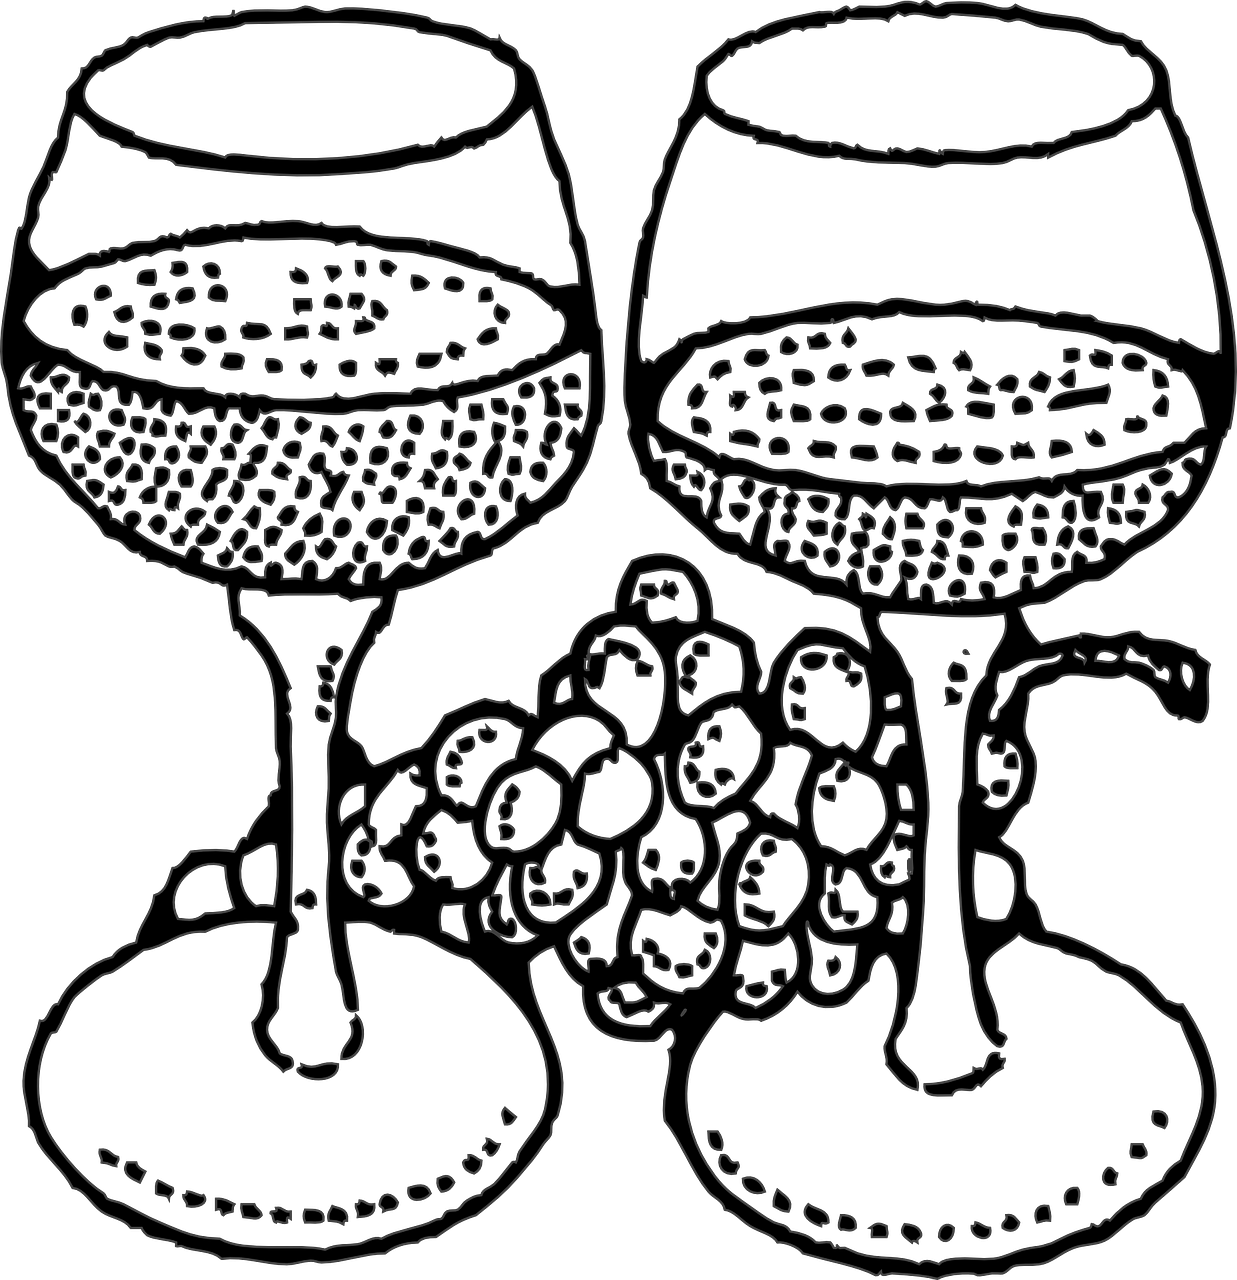
\includegraphics[width=0.2\textwidth]{images/brev83.png}
 \end{center}

\breakpage